\documentclass[10pt,letterpaper,final,twoside,notitlepage]{article}
\usepackage[margin=.5in]{geometry} % 1/2 inch margins on all pages
\usepackage[utf8]{inputenc} % Define the input encoding
\usepackage[USenglish]{babel} % Define language used
\usepackage{amsmath}
\usepackage{mathtools} % Allow for text and math in align* environment.
\usepackage{amsfonts}
\usepackage{amssymb}
\usepackage{amsthm} % Gives us plain, definition, and remark to use in \theoremstyle{style}
\usepackage{thmtools}
\usepackage{thm-restate}
\usepackage{graphicx}

\usepackage[
backend=biber,
style=alphabetic,
citestyle=authoryear]{biblatex} % Must include citation somewhere in document to print bibliography
\usepackage{hyperref} % Generate hyperlinks to referenced items
\usepackage[nottoc]{tocbibind} % Prints the Reference/Bibliography in TOC as well
\usepackage[noabbrev,nameinlink]{cleveref} % Fancy cross-references in the document everywhere
\usepackage{nameref} % Can make references by name to places
\usepackage{caption} % Allows for greater control over captions in figure, algorithm, table, etc. environments
\usepackage{subcaption} % Allows for multiple figures in one Figure environment
\usepackage[binary-units=true]{siunitx} % Gives us ways to typeset units for stuff
\usepackage{csquotes} % Context-sensitive quotation facilities
\usepackage{enumitem} % Provides [noitemsep, nolistsep] for more compact lists
\usepackage{chngcntr} % Allows us to tamper with the counter a little more
\usepackage{empheq} % Allow boxing of equations in special math environments
\usepackage[x11names]{xcolor} % Gives access to coloring text in environments or just text, MUST be before tikz
\usepackage{tcolorbox} % Allows us to create boxes of various types for examples
\usepackage{tikz} % Allows us to create TikZ and PGF Pictures
\usepackage{ctable} % Greater control over tables and how they look
\usepackage{multirow} % Allow us to have a single cell in a table span multiple rows
\usepackage{titling} % Put document information throughout the document programmatically
\usepackage[linesnumbered,ruled,vlined]{algorithm2e} % Allows us to write algorithms in a nice style.

\counterwithin{figure}{section}
\counterwithin{table}{section}
\counterwithin{equation}{section}
\counterwithin{algocf}{section}
\crefname{algocf}{algorithm}{algorithms}
\Crefname{algocf}{Algorithm}{Algorithms}
\setcounter{secnumdepth}{4}
\setcounter{tocdepth}{4} % Include \paragraph in toc
\crefname{paragraph}{paragraph}{paragraphs}
\Crefname{paragraph}{Paragraph}{Paragraphs}

% Create a theorem environment
\theoremstyle{plain}
\newtheorem{theorem}{Theorem}[section]
% Create a numbered theorem-like environment for lemmas
\newtheorem{lemma}{Lemma}[theorem]

% Create a definition environment
\theoremstyle{definition}
\newtheorem{definition}{Defn}
\newtheorem{corollary}{Corollary}[section]
% \begin{definition}[Term] \label{def:}
% 		Make sure the term is emphasized with \emph{term}.
%		This ensures that if \emph is changed, it shows up everywhere
% \end{definition}

% Create a numbered remark environment numbered based on definition
% NOTE: This version of remark MUST go inside a definition environment
\theoremstyle{remark}
\newtheorem{remark}{Remark}[definition]
%\counterwithin{definition}{subsection} % Uncomment to have definitions use section.subsection numbering

% Create an unnumbered remark environment for general use
% NOTE: This version of remark has NO restrictions on placement
\newtheorem*{remark*}{Remark}

% Create a special list that handles properties. It can be broken and restarted
\newlist{propertylist}{enumerate}{1} % {Name}{Template}{Max Depth}
% [newlistname, LevelsToApplyTo]{formatting options}
\setlist[propertylist, 1]{label=\textbf{(\roman*)}, ref=\textbf{(\roman*)}, noitemsep, nolistsep}
\crefname{propertylisti}{property}{properties}
\Crefname{propertylisti}{Property}{Properties}

% Create a special list that handles enumerate starting with lower letters. Breakable/Restartable.
\newlist{boldalphlist}{enumerate}{1} % {Name}{Template}{Max Depth}
% [newlistname, LevelsToApplyTo]{formatting options}
\setlist[boldalphlist, 1]{label=\textbf{(\alph*)}, ref=\alph*, noitemsep, nolistsep} % Set options

\newlist{nocrefenumerate}{enumerate}{1} % {Name}{Template}{Max Depth}
% [newlistname, LevelsToApplyTo]{formatting options}
\setlist[nocrefenumerate, 1]{label=(\arabic*), ref=(\arabic*), noitemsep, nolistsep}

% Create a list that allows for deeper nesting of numbers. By default enumerate only allows depth=4.
\newlist{nestednums}{enumerate}{6}
% [newlistname, LevelsToApplyTo]{formatting options}
\setlist[nestednums]{noitemsep, label*=\arabic*.}

\tcbuselibrary{breakable} % Allow tcolorboxes to be broken across pages
% Create a tcolorbox for examples
% /begin{example}[extra name]{NAME}
% Create a tcolorbox for examples
% Argument #1 is optional, given by [], that is the textbook's problem number
% Argument #2 is mandatory, given by {}, that is the title for the example
% Avoid putting special characters, (), [], {}, ",", etc. in the title.
\newtcolorbox[auto counter,
number within=section,
number format=\arabic,
crefname={example}{examples}, % Define reference format for cref (No Capitals)
Crefname={Example}{Examples}, % Reference format for cleveref (With Capitals)
]{example}[2][]{ % The [2][] Means the first argument is optional
  width=\textwidth,
  title={Example \thetcbcounter: #2. #1}, % Parentheses and commas are not well supported
  fonttitle=\bfseries,
  label={ex:#2},
  nameref=#2,
  colbacktitle=white!100!black,
  coltitle=black!100!white,
  colback=white!100!black,
  upperbox=visible,
  lowerbox=visible,
  sharp corners=all,
  breakable
}

% Create a tcolorbox for general use
\newtcolorbox[% auto counter,
% number within=section,
% number format=\arabic,
% crefname={example}{examples}, % Define reference format for cref (No Capitals)
% Crefname={Example}{Examples}, % Reference format for cleveref (With Capitals)
]{blackbox}{
  width=\textwidth,
  % title={},
  fonttitle=\bfseries,
  % label={},
  % nameref=,
  colbacktitle=white!100!black,
  coltitle=black!100!white,
  colback=white!100!black,
  upperbox=visible,
  lowerbox=visible,
  sharp corners=all
}

% Redefine the 'end of proof' symbol to be a black square, not blank
\renewcommand\qedsymbol{$\blacksquare$} % Change proofs to have black square at end

\renewcommand{\Re}{\operatorname{Re}} % Redefine to use the command, but not the fraktur version
\renewcommand{\Im}{\operatorname{Im}} % Redefine to use the command, but not the fraktur version
% Math Operators that are useful to abstract the written math away to one spot
\DeclareMathOperator{\RealNumbers}{\mathbb{R}}
\newcommand{\TextRealNumbers}{$\RealNumbers$}
\DeclareMathOperator{\AllIntegers}{\mathbb{Z}}
\newcommand{\TextAllIntegers}{$\AllIntegers$}
\DeclareMathOperator{\PositiveInts}{\mathbb{Z}^{+}}
\newcommand{\TextPositiveInts}{$\PositiveInts$}
\DeclareMathOperator{\NegativeInts}{\mathbb{Z}^{-}}
\newcommand{\TextNegativeInts}{$\NegativeInts$}
\DeclareMathOperator{\NaturalNumbers}{\mathbb{N}}
\newcommand{\TextNaturalNumbers}{$\NaturalNumbers$}
\DeclareMathOperator{\ComplexNumbers}{\mathbb{C}}
\newcommand{\TextComplexNumbers}{$\ComplexNumbers$}
\DeclareMathOperator{\RationalNumbers}{\mathbb{Q}}
\newcommand{\TextRationalNumbers}{$\RationalNumbers$}
\DeclareMathOperator*{\argmax}{argmax} % Thin Space and subscripts are UNDER in display
\DeclareMathOperator{\Lapl}{\mathcal{L}} % Declare a Laplace symbol to be used
\DeclareMathOperator{\UnitStep}{\mathcal{U}}
\DeclareMathOperator{\sinc}{sinc} % sinc(x) = (sin(pi x)/(pi x))
\DeclareMathOperator{\XOR}{\oplus}

\newcommand{\rbpRegister}{\texttt{\%rbp}}
\newcommand{\rspRegister}{\texttt{\%rsp}}
\newcommand{\ripRegister}{\texttt{\%rip}}
\newcommand{\raxRegister}{\texttt{\%rax}}
\newcommand{\rbxRegister}{\texttt{\%rbx}}

%%% Local Variables:
%%% mode: latex
%%% TeX-master: shared
%%% End:


% These packages are more specific to certain documents, but will be availabe in the template
% \usepackage{esint} % Provides us with more types of integral symbols to use
% \usepackage[outputdir=./TeX_Output]{minted} % Allow us to nicely typeset 300+ programming languages
% \crefname{lstlisting}{listing}{listings}
% \Crefname{lstlisting}{Listing}{Listings}
% This document must be compiled with the -shell-escape flag if the packages above are uncommented

\graphicspath{{./Drawings/MMAE_320-Thermo/}} % Uncomment this to use pictures in this document
% \addbibresource{./Bibliographies/CourseNum-Name.bib}

% Math Operators that are useful to abstract the written math away to one spot
% These are supposed to be document-specific mathematical operators that will make life easier
% Many fundamental operators are defined in Reference_Sheet_Preamble.tex
% Define English Imperial units.
% Define English Imperial units.
% Length
\DeclareSIUnit\inch{in}
\DeclareSIUnit\in{in}

\DeclareSIUnit\feet{ft}
\DeclareSIUnit\ft{ft}

\DeclareSIUnit\yard{yd}
\DeclareSIUnit\yd{yd}

\DeclareSIUnit\mile{mi}
\DeclareSIUnit\mi{mi}

% Volume
\DeclareSIUnit\fluidOunce{fl oz}
\DeclareSIUnit\floz{fl oz}

\DeclareSIUnit\pint{pt}
\DeclareSIUnit\pt{pt}

\DeclareSIUnit\quart{qt}
\DeclareSIUnit\qt{qt}

\DeclareSIUnit\gallon{gal}
\DeclareSIUnit\gal{gal}

% Mass
\DeclareSIUnit\grain{gr}
\DeclareSIUnit\gr{gr}

\DeclareSIUnit\ounce{oz}
\DeclareSIUnit\oz{oz}

\DeclareSIUnit\pound{lb}
\DeclareSIUnit\lb{lb}

\DeclareSIUnit\poundMass{lbm}
\DeclareSIUnit\lbm{lbm}

\DeclareSIUnit\ton{t}
\DeclareSIUnit\slug{slug}

% Temperature
\DeclareSIUnit\rankine{R}
\DeclareSIUnit[number-unit-product={}]\degreeF{\degree{}F}
\DeclareSIUnit[number-unit-product={}]\dF{\degree{}F}
\DeclareSIUnit[number-unit-product={}]\degF{\degree{}F}

\DeclareSIUnit[number-unit-product={}]\degreeR{\degree{}R}
\DeclareSIUnit[number-unit-product={}]\dR{\degree{}R}
\DeclareSIUnit[number-unit-product={}]\degR{\degree{}R}
% \DeclareSIUnit[number-unit-product={}]\Rankine{\degree{}R}
% \DeclareSIUnit[number-unit-product={}]\rankine{\degree{}R}
\DeclareSIUnit[number-unit-product={}]\degreeRankine{\degree{}R}

% Pressure
\DeclareSIUnit\bar{bar}
\DeclareSIUnit\atm{atm}
\DeclareSIUnit\psia{psia}
\DeclareSIUnit\psig{psig}
\DeclareSIUnit\psi{psi}

% Power
\DeclareSIUnit\horsepower{hp}
\DeclareSIUnit\hp{hp}

% Energy
\DeclareSIUnit\btu{btu}
\DeclareSIUnit\BTU{BTU}

%Force
\DeclareSIUnit\poundForce{lbf}
\DeclareSIUnit\lbf{lbf}

% volumetric flow
\DeclareSIUnit\cfm{cfm}
\DeclareSIUnit\CFM{CFM}

% Moles
\DeclareSIUnit\lbmol{lbmol}

%%% Local Variables:
%%% mode: latex
%%% TeX-master: shared
%%% End:


% By default, units should use the / symbol as the \per delimiter
% This can be overridden on a need-by-need basis though.
\sisetup{per-mode=symbol}

% Special Characters with Meaning
\newcommand{\Diameter}{\ensuremath{d}}
\newcommand{\Area}{\ensuremath{A}}
\newcommand{\Distance}{\ensuremath{d}}
\newcommand{\Density}{\ensuremath{\rho}}
\newcommand{\Pressure}{\ensuremath{P}}
\newcommand{\Temp}{\ensuremath{T}}
\newcommand{\Volume}{\ensuremath{V}}
\newcommand{\Mass}{\ensuremath{m}}
\newcommand{\Velocity}{\ensuremath{v}}
\newcommand{\Gravity}{\ensuremath{g}}
\newcommand{\Time}{\ensuremath{t}}
\newcommand{\GasConstant}{\ensuremath{R}}

\newcommand{\Energy}{\ensuremath{E}}
\newcommand{\TotalEnergy}{\ensuremath{E}}
\newcommand{\InternalEnergy}{\ensuremath{U}}
\newcommand{\SpecificInternalEnergy}{\ensuremath{u}}
\newcommand{\Heat}{\ensuremath{Q}}
\newcommand{\SpecificHeat}{\ensuremath{c}}
\newcommand{\SpecificHeatVolume}{\ensuremath{\SpecificHeat_{\Volume}}}
\newcommand{\SpecificHeatPressure}{\ensuremath{\SpecificHeat_{\Pressure}}}
\newcommand{\KineticEnergy}{\ensuremath{\mathrm{KE}}}
\newcommand{\PotentialEnergy}{\ensuremath{\mathrm{PE}}}
\newcommand{\FlowEnergy}{\ensuremath{\mathrm{FE}}}

\newcommand{\Efficiency}{\ensuremath{\eta}}

\newcommand{\Force}{\ensuremath{F}}
\newcommand{\Work}{\ensuremath{W}}
\newcommand{\Power}{\ensuremath{P}}

\newcommand{\SpecificWeight}{\ensuremath{\gamma_{s}}}
\newcommand{\SpecificVolume}{\ensuremath{\nu}}
\newcommand{\SpecificEnergy}{\ensuremath{e}}
\newcommand{\SpecificGravity}{\ensuremath{\mathrm{SG}}}

\newcommand{\Change}[1]{\ensuremath{\Delta #1}}
\newcommand{\FlowRate}[1]{\ensuremath{\dot{#1}}}

\newcommand{\Fluid}[1]{\ensuremath{#1_{f}}}
\newcommand{\Vapor}[1]{\ensuremath{#1_{g}}}
\newcommand{\FluidVapor}[1]{\ensuremath{#1_{fg}}}
\newcommand{\SaturatedFluidVol}{\ensuremath{\SpecificVolume_{f}}} % Can be V_{Fluid}
\newcommand{\SaturatedVaporVol}{\ensuremath{\SpecificVolume_{g}}} % Can be V_{Vapor} or V_{Gas}
\newcommand{\SaturatedPressure}{\ensuremath{\Pressure_{\mathrm{sat}}}}
\newcommand{\SaturatedTemp}{\ensuremath{\Temp_{\mathrm{sat}}}}
\newcommand{\Quality}{\ensuremath{x}}

% Saturated Mixture (Specific) Internal Energies
\newcommand{\SaturatedFluidIntEnergy}{\ensuremath{\InternalEnergy_{f}}}
\newcommand{\SaturatedVaporIntEnergy}{\ensuremath{\InternalEnergy_{g}}}
\newcommand{\SaturatedFluidVaporIntEnergy}{\ensuremath{\InternalEnergy_{fg}}}
\newcommand{\SaturatedFluidSpecificIntEnergy}{\ensuremath{\SpecificInternalEnergy_{f}}}
\newcommand{\SaturatedVaporSpecificIntEnergy}{\ensuremath{\SpecificInternalEnergy_{g}}}
\newcommand{\SaturatedFluidVaporSpecificIntEnergy}{\ensuremath{\SpecificInternalEnergy_{fg}}}

\newcommand{\Enthalpy}{\ensuremath{H}}
\newcommand{\SpecificEnthalpy}{\ensuremath{h}}
% Specific Mixture (Specific) Enthalpy
\newcommand{\SaturatedFluidEnthalpy}{\ensuremath{\Enthalpy_{f}}}
\newcommand{\SaturatedVaporEnthalpy}{\ensuremath{\Enthalpy_{g}}}
\newcommand{\SaturatedFluidVaporEnthalpy}{\ensuremath{\Enthalpy_{fg}}}
\newcommand{\SaturatedFluidSpecificEnthalpy}{\ensuremath{\SpecificEnthalpy_{f}}}
\newcommand{\SaturatedVaporSpecificEnthalpy}{\ensuremath{\SpecificEnthalpy_{g}}}
\newcommand{\SaturatedFluidVaporSpecificEnthalpy}{\ensuremath{\SpecificEnthalpy_{fg}}}

\begin{titlepage}
  \title{MMAE 320: Thermofluid Dynamics --- Reference Material \\ Illinois Institute of Technology}
  \author{Karl Hallsby}
  \date{Last Edited: \today} % We want to inform people when this document was last edited
\end{titlepage}

\begin{document}
\pagenumbering{gobble}
\maketitle
\pagenumbering{roman} % i, ii, iii on beginning pages, that don't have content
\tableofcontents
\clearpage
\listoftheorems[ignoreall, show={definition, Definition}]
\clearpage
\pagenumbering{arabic} % 1,2,3 on content pages

\section{Introduction}\label{sec:Introduction}

%%% Local Variables:
%%% mode: latex
%%% TeX-master: "../MMAE_320-Thermo-Reference_Sheet"
%%% End:


\section{Basic Concepts}\label{sec:Basic_Concepts}

\subsection{Systems}\label{subsec:Systems}
\begin{definition}[System]\label{def:System}
  A \emph{system} is defined as a quantity of matter or a region in space chosen for study.
\end{definition}

The mass or region outside the \nameref{def:System} is the \textbf{surroundings}.
The surface that separates the \nameref{def:System} from the surroundings is the \textbf{boundary}.


%%% Local Variables:
%%% mode: latex
%%% TeX-master: "../../MMAE_320-Thermo-Reference_Sheet"
%%% End:


%%% Local Variables:
%%% mode: latex
%%% TeX-master: "../MMAE_320-Thermo-Reference_Sheet"
%%% End:

\section{Energy, and Energy Transfer}\label{sec:Energy_Energy_Transfer}
\begin{definition}[Macroscopic Energy Form]\label{def:Macroscopic_Energy_Form}
  \emph{Macroscopic energy form}s are typically ones that have to deal with objects on a macroscopic level.
  These energies are:
  \begin{enumerate}[noitemsep]
  \item Kinetic
  \item Potential
  \end{enumerate}

  \begin{remark}
    This definition is included because the textbook makes use of it.
  \end{remark}
\end{definition}

\begin{definition}[Microscopic Energy Form]\label{def:Microscopic_Energy_Form}
  \emph{Microscopic energy forms} are energies that act on non-macroscopic levels.
  Namely, they affect their systems on microscopic levels.
  These energies include:
  \begin{enumerate}[noitemsep]
  \item Sensible
    \begin{itemize}[noitemsep]
    \item Heat
    \item Kinetic energy of molecules
    \end{itemize}
  \item Latent
    \begin{itemize}[noitemsep]
    \item Phase Changes
    \end{itemize}
  \item Chemical
    \begin{itemize}[noitemsep]
    \item Combustion
    \end{itemize}
  \item Nuclear
  \end{enumerate}

  \begin{remark}
    This definition is included because the textbook makes use of it.
  \end{remark}
\end{definition}

\begin{definition}[Internal Energy]\label{def:Internal_Energy}
  \emph{Internal energy} is equivalent to \nameref{def:Microscopic_Energy_Form}s.
  It means the \nameref{def:Energy} that the object in question inherently has at that point in time.
\end{definition}

\subsection{Energy Quality}\label{subsec:Energy_Quality}
Energy has quality!
\begin{itemize}[noitemsep]
\item \nameref{def:Macroscopic_Energy_Form}
  \begin{itemize}[noitemsep]
  \item Structured
  \item Moves as a single unit
  \end{itemize}
\item \nameref{def:Microscopic_Energy_Form}
  \begin{itemize}[noitemsep]
  \item \textbf{Not} structures
  \item Does \textbf{not} move as a single unit
  \end{itemize}
\end{itemize}

These differences mean that we measure the efficiency of each type of energy form differently.

\subsection{Energy and Flows}\label{subsec:Energy_and_Flows}
When moving a fluid through a pipe, we can find the amount of work done by the fluid flowing, called teh \nameref{def:Flow_Energy}.
\begin{align*}
  \Pressure &= \frac{\Force}{\text{Area}} \\
  \Volume_{\mathrm{Cylinder}} &= \ell \cdot \text{Area} \\
  \Work &= \Force \cdot \text{Distance} \\
\end{align*}

If we substitute for the common terms in the formula for work, then we end up with \Cref{eq:Flow_Energy}.

\begin{definition}[Flow Energy]\label{def:Flow_Energy}
  \emph{Flow energy} is the energy that a fluid flowing through a long, straight pipe has.

  \begin{equation}\label{eq:Flow_Energy}
    \begin{aligned}
      \Work &= \Pressure \Volume \\
      \FlowEnergy &= \Pressure \Volume \\
    \end{aligned}
  \end{equation}

  \begin{remark}[Energy Form]
    Typically, \nameref{def:Flow_Energy} is categorized with the \nameref{def:Macroscopic_Energy_Form}s, because it behaves more like those and can be nearly as efficient as them.
    This is true even though this is technically an application of microscopic energies.
    This is because we are not worried about the internal energy of the fluid in the pipe, but are instead interested in the mechanical movement of it.
  \end{remark}
\end{definition}

\subsection{Divisions of Energy}\label{subsec:Divisions_of_Energy}
We are always interested in the change in energy that occurs due to something.
This is seen as \Cref{eq:Change_Total_Energy}.

\begin{equation}\label{eq:Change_Total_Energy}
  \begin{aligned}
    \Change{\TotalEnergy} &= \Change{\InternalEnergy} + \Change{\KineticEnergy} + \Change{\PotentialEnergy} + \Change{\FlowEnergy} \\
    &= \frac{\InternalEnergy_{2} - \InternalEnergy_{1}}{\Mass} + \frac{v_{2}^{2} - v_{1}^{2}}{2} + \Gravity (h_{2} - h_{1}) + \frac{\Pressure_{2} - \Pressure_{1}}{\Density} \\
  \end{aligned}
\end{equation}
\begin{itemize}[noitemsep]
\item The internal energy cannot be completely converted into work.
\item Mechanical energy is typically defined to be these types of energies.
  These can be completely converted into work by an ideal machine.
  \begin{itemize}[noitemsep]
  \item Kinetic energy ($\KineticEnergy$)
  \item Potential energy ($\PotentialEnergy$)
  \item Flow energy ($\FlowEnergy$)
  \end{itemize}
\end{itemize}

We are also interested in the \nameref{def:Specific_Energy} of the system.
\begin{definition}[Specific Energy]\label{def:Specific_Energy}
  \emph{Specific energy} is an \nameref{def:Intensive_Property} of a system.
  It is the total energy of a system divided by the total mass of the system.
  \begin{equation}\label{eq:Specific_Energy}
    \begin{aligned}
      \SpecificEnergy &= \frac{\TotalEnergy}{\Mass} \\
      &= \frac{\InternalEnergy}{\Mass} + \frac{1}{2} v^{2} + \Gravity h + \frac{\Pressure \Volume}{\Mass} \\
      &= \frac{\InternalEnergy}{\Mass} + \frac{1}{2} v^{2} + \Gravity h + \frac{\Pressure}{\Density} \\
    \end{aligned}
  \end{equation}
\end{definition}

The \nameref{def:Specific_Energy} of a system can be used to find the change in energy per unit time, or the \nameref{def:Power}.
\begin{equation}\label{eq:Energy_Flow_Rate}
  \begin{aligned}
    \Change{\FlowRate{\TotalEnergy}} &= \FlowRate{\Mass} \Change{\SpecificEnergy} \\
    \Power &= \FlowRate{\Mass} \Change{\SpecificEnergy} \\
  \end{aligned}
\end{equation}
where $\FlowRate{\Mass}$ is the mass flow rate, seen by \Cref{eq:Mass_Flow_Rate}

\begin{equation}\label{eq:Mass_Flow_Rate}
  \FlowRate{\Mass} = \frac{\Mass}{\Time}
\end{equation}


%%% Local Variables:
%%% mode: latex
%%% TeX-master: "../MMAE_320-Thermo-Reference_Sheet"
%%% End:


\section{Properties of Pure Substances}\label{sec:Properties_Pure_Substances}
Many of the substances that we study in \nameref{def:Thermodynamics} are what we call \nameref{def:Pure_Substance}s.

\begin{definition}[Pure Substance]\label{def:Pure_Substance}
  A \emph{pure substance} is one whose chemical composition is fixed throughout.
  Properties of these substances are completely known, and these properties are completely uniform throughout the substance.
\end{definition}

In general, the pressure of a substance is an exponential function that is dependent on the temperature of the water.
In addition, the pressure of the substance depends on its altitude.
As you increase in altitude, this means that the temperature required to boil the substance at decreases.
All of these are visualized in \Cref{fig:Temp_Pressure_Liquid_Vapor_Curve}.

\begin{figure}[h!tbp]
  \centering
  \includegraphics[scale=0.75]{./Temperature_Pressure_Liquid_Vapor_Curve.png}
  \caption{Temperature-Pressure ($\Temp$-$\Pressure$) Liquid-Vapor Curve}
  \label{fig:Temp_Pressure_Liquid_Vapor_Curve}
\end{figure}

\subsection{Phase Changes}\label{subsec:Phase_Changes}
Phase changes in materials are unique, because they maintain a constant temperature \textbf{until} all the material undergoes the phase change, however, the volume increases \textbf{drastically}.

\begin{definition}[Phase Change]\label{def:Phase_Change}
  A \emph{phase change} in a substance is when it changes from one state of matter to another.
  This means a substance goes from solid to liquid, liquid to gas, gas to solid, solid to gas, etc.
  Each of these ``directions'' has a name:
  \begin{description}[noitemsep]
  \item[Solid to Liquid:] Melting/Fusion
  \item[Liquid to Solid:] Solidification/Crystallization
  \item[Liquid to Gas:] Evaporation/Vaporization
  \item[Gas to Liquid:] Condensation
  \item[Solid to Gas:] Sublimation
  \item[Gas to Solid:] Desposition
  \end{description}
\end{definition}

This is visualized as the line between points $A$ and $B$ on the graph in \Cref{fig:Phase_Change}.

\begin{figure}[h!tbp]
  \centering
  \includegraphics[scale=0.65]{./Phase_Change_Graph.png}
  \caption{Phase Change Graph}
  \label{fig:Phase_Change}
\end{figure}

The line drawn in \Cref{fig:Phase_Change} assumes that the material undergoing the phase change is under \nameref{def:Isobaric} conditions, meaning the pressure is \textbf{not} changing.
However, different pressures (under their own \nameref{def:Isobaric} conditions) will yield different, but similarly shaped, lines as well.

\begin{remark*}
  \Cref{fig:Phase_Change} is also \textbf{NOT} drawn to proportion, as the angle on the first portion of the line is typically \textbf{very} sharp.
  Obviously, \Cref{fig:Phase_Change} is an idealized graph for the temperature-volume graph of a substance and its respective phase change.
  Even though the graph is idealized, it is fine for our needs, and for most needs in \nameref{def:Thermodynamics}.
\end{remark*}


%%% Local Variables:
%%% mode: latex
%%% TeX-master: "../MMAE_320-Thermo-Reference_Sheet"
%%% End:


\section{Energy Analysis of \nameref*{def:Closed_System}s}\label{def:Energy_Analysis_Closed_Systems}
Gases can perform work, meaning they can expend \nameref{def:Energy}.

For example, in a piston, there is a contained gas, which can press one side up and out.
Remember the equation for \nameref{def:Work}, \Cref{eq:Work}.
But, because we are dealing with gas pressures, we rewrite \Cref{eq:Work}.
\begin{align*}
  \Work &= \Pressure \Area \Distance \\
  \Delta \Work &= \Pressure \Area \Delta \Distance \\
        &= \Pressure \Delta \Volume \\
  \intertext{We can express the change in work using differentials too, so we can integrate.}
  d \Work &= \Pressure d\Volume
\end{align*}


\begin{definition}[Specific Enthalpy]\label{def:Specific_Enthalpy}
  \emph{Specific enthalpy} is also commonly referred to as just \emph{enthalpy}, as context makes clear which one is being discussed.
  Specific enthalpy is the total \nameref{def:Heat} content of a \nameref{def:System} per unit mass of that system.
  Specific Enthalpy is defined in \Cref{eq:Specific_Enthalpy}.
  \begin{equation}\label{eq:Specific_Enthalpy}
    \SpecificEnthalpy = \SpecificInternalEnergy + \Pressure \SpecificVolume \:\: \si{\joule\per\gram}
  \end{equation}
\end{definition}

\begin{definition}[Enthalpy]\label{def:Enthalpy}
  \emph{Enthalpy} is the total \nameref{def:Heat} content of a \nameref{def:System}.
  It is equal to the \nameref{def:Internal_Energy} of the system plus the product of \nameref{def:Pressure} and volume.
  \begin{equation}\label{eq:Enthalpy}
    \Enthalpy = \InternalEnergy + \Pressure \Volume \:\: \si{\joule}
  \end{equation}
\end{definition}

%%% Local Variables:
%%% mode: latex
%%% TeX-master: "../MMAE_320-Thermo-Reference_Sheet"
%%% End:


\section{Mass and Energy Analysis of Control Volumes}\label{sec:Mass_Energy_Analysis_Control_Volumes}
\subsection{Continuity Equation}\label{subsec:Continuity_Equation}
We perform this analysis when we are interested in the matter flow of a \nameref{def:System}.
We still need to have \nameref{def:Law_Conservation_Energy}.
The important thing to remember here is that there is no change of mass of the control volume, meaning there is \textbf{no} storage of the mass in the system.
This means we have \emph{steady flow}.
This also means we could have an unsteady flow, but we deal with that later in this section.

Now, to motivate the \nameref{def:Continuity_Equation}, imagine an expandable tank.
If there are $n$ flows inwards and $m$ flows outwards, we can construct an equation that looks like this.
\begin{align*}
  (\FlowRate{\Mass_{In,1}} + \FlowRate{\Mass_{In,2}}) - \FlowRate{\Mass_{Out}} &= {\left[ \frac{dm}{dt} \right]}_{\text{Control Volume}} \\
  \sum\limits_{\text{Inlets}} \FlowRate{\Mass} - \sum\limits_{\text{Outlets}} \FlowRate{\Mass} &= \FlowRate{\Mass}_{\text{Control Volume}}
\end{align*}

\begin{definition}[Continuity Equation]\label{def:Continuity_Equation}
  The \emph{continuity equation} states the relationship between the mass flow into a point in a \nameref{def:System} and its output.
  Succinctly, it can be stated:
  \begin{equation}\label{eq:Continuity_Equation}
    \begin{aligned}
      \sum\limits_{\text{Inlets}} \FlowRate{\Mass} - \sum\limits_{\text{Outlets}} \FlowRate{\Mass} &= \FlowRate{\Mass}_{\text{Control Volume}} \\
      \sum\limits_{\text{Inlets}} \FlowRate{\Volume} - \sum\limits_{\text{Outlets}} \FlowRate{\Volume} &= \FlowRate{\Volume}_{\text{Control Volume}}
    \end{aligned}
  \end{equation}

  \begin{description}[noitemsep]
  \item $\FlowRate{\Mass}_{\text{Control Volume}}$ is the storage possible in a vessel, in mass.
    Likewise, $\FlowRate{\Volume}_{\text{Control Volume}}$ is the possible storage of a vessel, in volume.
  \end{description}

  \begin{remark}[Alternate Definitions of Mass Flowrate]\label{rmk:Alternative_Mass_Flowrate_Defns}
    It will be useful to remember alternative versions of mass flowrate for this particular section.
    Namely,
    \begin{align*}
      \FlowRate{\Mass}_{1} &= \FlowRate{\Mass}_{2} \\
      \Density_{1} \Velocity_{1} \Area_{1} &= \Density_{2} \Velocity_{2} \Area_{2}
    \end{align*}
  \end{remark}
\end{definition}

There are 2 situations that can arise from the \nameref{def:Continuity_Equation}.
\begin{enumerate}[noitemsep]
\item Rigid control volumes, $\FlowRate{\Mass}_{\text{Control Volume}} = 0$.
\item Non-rigid control volumes, $\FlowRate{\Mass}_{\text{Control Volume}} \neq 0$.
\end{enumerate}

\begin{example}{Use Continuity Equation}
  A nozzle is attached to a \SI{20}{\gallon} bucket to fill it.
  The inner diameter of the hose is \SI{1}{\inch} and reduces to \SI{0.5}{\inch} at the nozzle's exit.
  If the average velocity of the water in the hose is \SI{8}{\feet\per\second} determine the volume and mass flow rates, $\FlowRate{\Volume}$ and $\FlowRate{\Mass}$ of the water through the hose and how long it will take to fill the bucket?
  Also determine the average velocity at the tip of the nozzle, $\Velocity_{Out}$?
  \tcblower{}
  \textbf{Concepts:} \\
  A nozzle has 1 inlet and 1 outlet.
  The diameter of the nozzle at the inlet is $\Diameter_{In} = \SI{1}{\inch}$, and the outlet $\Diameter_{Out} = \SI{0.5}{\inch}$. \\
  There is no temperature change in the hose, so the density of the water is constant, $\Change{\Density_{Water}} = 0$. \\
  Because the host does not have any storage, $\FlowRate{\Mass}_{\text{Control Volume}} = 0$.
  Therefore, $\FlowRate{\Mass}_{In} = \FlowRate{\Mass}_{Out}$ and $\FlowRate{\Volume}_{In} = \FlowRate{\Volume}_{Out}$.

  \textbf{Explore:} \\
  $\Density_{\text{Water}} = \SI{62.3}{\lbm\per\feet\cubed}$, as \SI{32}{\degreeF}. \\
  The bucket has a capacity of \SI{20}{\gallon}, which means $20 = \FlowRate{\Volume} \times \text{Time to fill}$.

  \textbf{Plan:} \\
  Solve for $\FlowRate{\Volume}$, $\FlowRate{\Mass}$, $\Volume_{2}$.

  \textbf{Solve:} \\
  Start with a definition of volume flowrate.
  \begin{align*}
    \FlowRate{\Volume}_{In} &= \Area_{In} \Velocity_{In} \\
                            &= \frac{\pi \Diameter_{In}^{2}}{4} \SI{8}{\feet\per\second} \\
                            &= \SI{0.0436}{\cubic\feet\per\second}
  \end{align*}

  Now, we can find the mass flowrate through the inlet of the hose.
  \begin{align*}
    \FlowRate{\Mass} &= \Density_{Water} \FlowRate{\Volume} \\
                     &= \SI{62.3}{\lbm\per\feet\cubed} (\SI{0.0436}{\cubic\feet\per\second}) \\
                     &= \SI{2.72}{\lbm\per\second}
  \end{align*}

  Because the flowrates at the inlet and outlet of the hose are the same, we can reuse these values to solve for the time to fill the bucket.
  \begin{align*}
    \SI{20}{\gallon} \frac{\SI{1}{\cubic\feet}}{\SI{7.48}{\gallon}} &= \FlowRate{\Volume} \Time \\
    \Time &= \SI{61.3}{\second}
  \end{align*}

  Lastly, we need to solve for the velocity of the flowing water at the tip of the nozzle.
  We can use the relation between mass flowrates, shown in \Cref{rmk:Alternative_Mass_Flowrate_Defns}.
  \begin{align*}
    \Density_{Water} \Area_{In} \Velocity_{In} &= \Density_{Water} \Area_{Out} \Velocity_{Out} \\
    \Area_{In} \Velocity_{In} &= \Area_{Out} \Velocity_{Out} \\
    \Velocity_{Out} &= \frac{\Area_{In} \Velocity_{In}}{\Area_{Out}} \\
                                               &= \frac{\frac{\pi \Diameter_{In}^{2}}{4} \Velocity_{In}}{\frac{\pi \Diameter_{Out}^{2}}{4}} \\
    \Velocity_{Out} &= \SI{32}{\feet\per\second}
  \end{align*}

  \textbf{Validate:} \\
  We can validate that our answer for volume flowrate makes sense by multiplying the outlet volume flowrate by the outlet velocity and the outlet cross-sectional area.
  \begin{align*}
    \FlowRate{\Volume}_{Out} &= \Velocity_{Out} \times \Area_{Out} \\
                             &= \SI{32}{\feet\per\second} \frac{\pi \Diameter_{Out}^{2}}{4} \\
  \end{align*}

  If we look at this closely, we notice that when the diameter of the outlet was halved, the total area was quartered.
  Correspondingly, there was a four times increase in the velocity of the water at the outlet.

  \textbf{Generalize:} \\
  Constant mass flow and constant fluid density reuislts in a change at the outlet based on the change in area.
\end{example}

%%% Local Variables:
%%% mode: latex
%%% TeX-master: "../../MMAE_320-Thermo-Reference_Sheet"
%%% End:


\subsection{Energy Flows}\label{subsec:Energy_Flows}
\begin{table}[h!tbp]
  \centering
  \begin{tabular}{ccccc}
    \toprule
    & \nameref{def:Internal_Energy} & Kinetic Energy & Potential Energy & \nameref{def:Flow_Energy} \\
    \midrule
    \nameref{def:Specific_Energy}, $\SpecificEnergy$ & $\SpecificInternalEnergy$ & $\frac{\Velocity^{2}}{2}$ & $\Gravity \Distance$ & $\frac{\Pressure}{\Density}$ \\
    \nameref{def:Energy}, $\Energy$ & $\InternalEnergy$ & $\frac{\Mass \Velocity^{2}}{2}$ & $\Mass \Gravity \Distance$ & $\Pressure \Volume$ \\
    \bottomrule
  \end{tabular}
  \caption{Types of Energy for Mass Flow}
  \label{tab:Energy_Flows}
\end{table}


%%% Local Variables:
%%% mode: latex
%%% TeX-master: "../../MMAE_320-Thermo-Reference_Sheet"
%%% End:


%%% Local Variables:
%%% mode: latex
%%% TeX-master: "../MMAE_320-Thermo-Reference_Sheet"
%%% End:


\section{The Second Law of Thermodynamics}\label{sec:2nd_Law_Thermo}
\begin{definition}[\nth{2} Law of Thermodynamics]\label{def:2nd_Law_Thermo}
  The \emph{\nth{2} law of thermodynamics} states that the total \nameref{def:Entropy} of an \nameref{def:Isolated_System} can \textbf{never} decrease over time, and is constant if and only if all \nameref{def:Process}es are reversible.
  Isolated systems spontaneously evolve towards thermodynamic equilibrium, the state with maximum entropy.

  In terms of total \nameref{def:Energy} in a system, this law states that the total energy of the system is minimized at all times during a \nameref{def:Process}.

  \begin{remark}
    We do not discuss \nameref{def:Entropy} in this section.
    Rather, we discuss it in great detail in \Cref{sec:Entropy}.
  \end{remark}
\end{definition}

In more common terms, the \nameref{def:2nd_Law_Thermo} explains why some \nameref{def:Process}es only move in one direction.
For example, water going over a waterfall is \textit{technically} symmetric.
Meaning, that there is a chance the water will actually go back \textbf{up} the cliff.
However, the \nameref{def:2nd_Law_Thermo} explains that this reversal is so thermodynamically unfavorable that it will never happen.

Another example is a container of water that is greater than that of its surroundings.
For instance, the water is $\Temp = \SI{90}{\degreeF}$ and the surroundings are at $\Temp = \SI{20}{\degreeF}$.
The \nameref{def:2nd_Law_Thermo} explains why the heat always flows \textbf{out} of the water and to the surroundings, rather than the other way around.

This means that \textbf{energy is dispersed}.
This spread (dispersion) of energy is \nameref{def:Entropy}.

%%% Local Variables:
%%% mode: latex
%%% TeX-master: "../MMAE_320-Thermo-Reference_Sheet"
%%% End:


%====================================APPENDIX====================================
\appendix
\counterwithin{definition}{subsection}

\clearpage
\section{Complex Numbers}
	\begin{equation} \label{eq:Exponential to Rectangular}
		A e^{-ix} = A \left[ \cos \left( x \right) + i\sin \left( x \right) \right]
	\end{equation}

\clearpage
\subsection{Trigonometry} \label{app:Trig}
	\subsubsection{Trigonometric Formulas} \label{subsubsec:Trig Formulas}
		\begin{equation} \label{eq:Sin plus Sin with diff Angles}
			\sin \left( \alpha \right) + \sin \left( \beta \right) = 2 \sin \left( \frac{\alpha + \beta}{2} \right) \cos\left( \frac{\alpha - \beta}{2} \right)  
		\end{equation}
		\begin{equation} \label{eq:Cosine-Sine Product}
			\cos \left( \theta \right) \sin \left( \theta \right) = \frac{1}{2} \sin \left( 2 \theta \right)
		\end{equation}

\clearpage
\subsection{Calculus} \label{app:Calculus}
	\subsubsection{Fundamental Theorems of Calculus} \label{subsubsec:Fundamental Theorem of Calculus}
		\begin{definition}[First Fundamental Theorem of Calculus] \label{def:1st Fundamental Theorem of Calculus}
			The \emph{first fundamental theorem of calculus} states that, if $f$ is continuous on the closed interval $\left[ a,b \right]$ and $F$ is the indefinite integral of $f$ on $\left[ a,b \right]$, then 
			\begin{equation} \label{eq:1st Fundamental Theorem of Calculus}
				\int_{a}^{b}f \left( x \right) dx = F \left( b \right) - F \left( a \right)
			\end{equation}
		\end{definition}
		\begin{definition}[Second Fundamental Theorem of Calculus] \label{def:2nd Fundamental Theorem of Calculus}
			The \emph{second fundamental theorem of calculus} holds for $f$ a continuous function on an open interval $I$ and $a$ any point in $I$, and states that if $F$ is defined by
			\begin{equation*}
				F \left( x \right) = \int_{a}^{x} f \left( t \right) dt,
			\end{equation*}
			then
			\begin{equation} \label{eq:2nd Fundamental Theorem of Calculus}
				\begin{aligned}
					\frac{d}{dx} \int_{a}^{x} f \left( t \right) dt &= f \left( x \right) \\
					F' \left( x \right) &= f \left( x \right) \\
				\end{aligned}
			\end{equation}
		\end{definition}

\clearpage
\section{Laplace Transform}\label{app:Laplace_Transform}
\subsection{Laplace Transform}\label{subsec:Laplace_Transform}
\begin{definition}[Laplace Transform]\label{def:Laplace_Transform}
  The \emph{Laplace transformation} operation is denoted as $\Lapl \lbrace x(t) \rbrace$ and is defined as
  \begin{equation}\label{eq:Laplace_Transform}
    X(s) = \int\limits_{-\infty}^{\infty} x(t) e^{-st} dt
  \end{equation}
\end{definition}

\subsection{Inverse Laplace Transform}\label{subsec:Inverse_Laplace_Transform}
\begin{definition}[Inverse Laplace Transform]\label{def:Inverse_Laplace_Transform}
  The \emph{inverse Laplace transformation} operation is denoted as $\Lapl^{-1} \lbrace X(s) \rbrace$ and is defined as
  \begin{equation}\label{eq:Inverse_Laplace_Transform}
    x(t) = \frac{1}{2j \pi} \int_{\sigma-\infty}^{\sigma+\infty} X(s) e^{st} \, ds
  \end{equation}
\end{definition}



% To make this print, you must include a citation somewhere in the document
\clearpage
\printbibliography{}
\end{document}

%%% Local Variables:
%%% mode: latex
%%% TeX-master: t
%%% End:
